\section{Introduction}

Blockchain oracles supply smart contracts with information that the ledger cannot observe. Prices and event outcomes enter contract execution through reporting, verification and dispute resolution~\cite{zhang2016towncrier,eskandari2021sok}. Participants may earn rewards, post capital, challenge reports or incur penalties. These arrangements determine both the information a contract accepts and the incentives for providing it~\cite{cong2019blockchain,cong2025oracleprimer}.

Public transactions do not make these incentives directly measurable. A transfer may combine returned principal with a reward; a negative accounting adjustment may precede any reduction in stake. Disputed requests can traverse several contracts or chains, whose versions, identifiers and accounting rules differ. Treating gross payouts as profit or accruals as realized losses changes the economic quantity being measured. Comparison requires lifecycle reconstruction under the applicable protocol rules.

Oracle mechanisms expose different aspects of economic accountability: proposals and adjudication, staking operations, reward epochs, signed updates or withdrawals. Oracle4SD Atlas selects branches for this variation and the historical evidence available to reconstruct it. The sample supports comparisons of specified activities; it is neither a census of oracle services nor a probability sample of the ecosystem.

The resource covers eight branches: five detailed panels for UMA, Chainlink, Tellor, Flare FTSOv2 and Pyth, and three narrower extensions for Chronicle, RedStone Push and DIA. The common accountability representation contains 105,588,120 typed observations, complemented by 22,723,389 economic components and 19,275,854 records meeting protocol-specific realization criteria. These representations overlap and use different observation units, so their counts cannot be added. Native records accompany the common fields, linking comparative measures to their supporting evidence.

The contribution is a measurement framework that connects protocol rules and native records to observable economic states. By distinguishing configured incentives, accrued adjustments, claimable entitlements, realized payments and applied losses, the resource supports descriptive research on participation, incentives and accountability within documented coverage boundaries. Figure~\ref{fig:ecosystem_scope} situates the sampled implementations within the wider oracle ecosystem, while Table~\ref{tab:protocol_sources} summarizes the scope of each branch. Comparisons remain conditional on observation units, historical rules and evidence availability. Protocol acceptance and financial execution are therefore interpreted separately from independent verification of external facts.

\begin{figure}[!htbp]
\centering
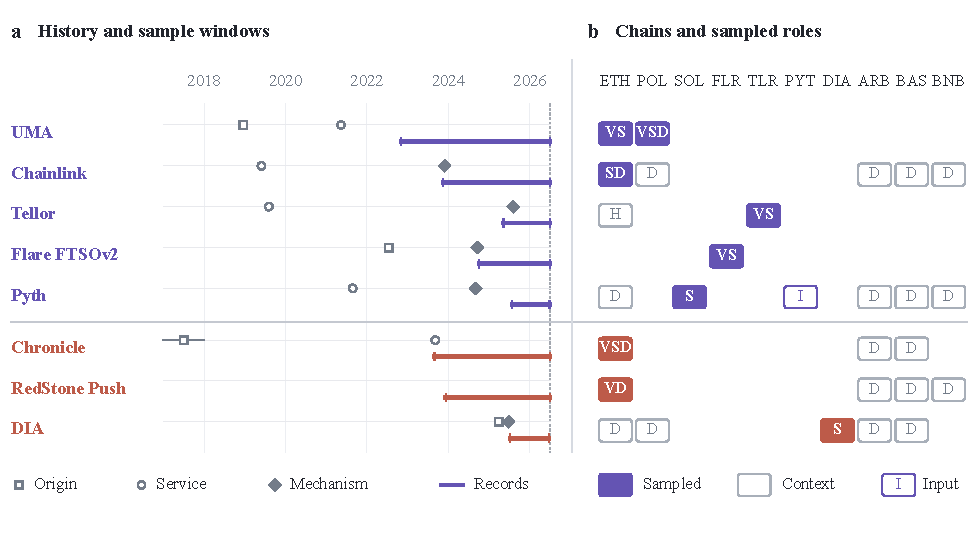
\includegraphics[width=\linewidth]{figures/ecosystem_scope.pdf}
\caption{Historical context and sampled scope of Oracle4SD Atlas. Purple denotes five detailed panels; coral denotes three narrower extensions. (a) Symbols mark project or network origins, service openings, and mechanism announcements or access milestones. Coloured segments delimit retained timestamps in one selected table per branch; they do not imply uninterrupted acquisition. The dashed line marks the 30 June 2026 cutoff. (b) Filled cells identify sampled chain roles; grey outlines show selected ecosystem context. V, verification/adjudication; S, economic settlement/accounting; D, delivery; H, historical implementation; I, retained derived inputs. ETH, Ethereum; POL, Polygon; SOL, Solana; FLR, Flare; TLR, tellor-1; PYT, Pythnet; DIA, Lasernet; ARB, Arbitrum; BAS, Base; BNB, BNB Chain. Dates and source evidence are provided in Appendix~\ref{app:scope}.}
\label{fig:ecosystem_scope}
\end{figure}


\section{Related work}

Research on oracles and research on blockchain datasets approach the same infrastructure from complementary directions. Oracle studies examine how external information is authenticated, aggregated and incentivized; data-resource studies establish reusable representations of transactions, entities and contracts. The present work connects these perspectives by making the relationship between native protocol evidence and economic measurement explicit. Tables~\ref{tab:oracle_related_work} and~\ref{tab:blockchain_datasets} summarize representative contributions without treating their differing units or purposes as directly comparable measures of scale.

\subsection{Oracle design, security and economic institutions}

Town Crier authenticates external data delivery through trusted hardware; DECO proves properties of data obtained over TLS~\cite{zhang2016towncrier,zhang2020deco}. The oracle systematization of knowledge reviews trust assumptions, attacks and mitigations~\cite{eskandari2021sok}. Adaptive conformal consensus provides conditional guarantees for aggregating reports, while SMARTCAT detects contracts associated with price-manipulation attacks~\cite{park2023acon,zhang2025smartcat}. These studies address information security; we reconstruct participant incentives and economic outcomes.

Empirical oracle studies provide a second foundation. A first look at DeFi oracles measures deployed price-oracle behavior, while Demystifying Pythia examines Chainlink usage, pricing and service quality on Ethereum~\cite{liu2021firstlook,kaleem2021pythia}. Economic research complements these observations by analyzing incentives, staking, decentralization and the integration of oracle networks with financial markets~\cite{cong2025oracleprimer,cong2026integration}. Together, these studies motivate an empirical representation that follows the economic process across participation, challenge, adjudication and settlement. The framework developed here retains those stages where the source evidence supports them, rather than assuming that every mechanism exposes an equivalent lifecycle.

The mechanisms represented in the Atlas expose different empirical objects. UMA and Tellor provide settings for studying contestable reporting, challenge participation and adjudicated outcomes~\cite{uma2026,tellorDisputes2026}. Chainlink's staking and feed records distinguish economic participation from observable service updates~\cite{chainlinkstaking2026}, while Flare FTSOv2 separates reward entitlements, provider conditions and subsequent claims~\cite{flareFTSO2026}. Pyth's OIS records connect publisher-related incentive states with staking operations and economic transfers within the retained historical window~\cite{pythOIS2026}. The narrower Chronicle, RedStone Push and DIA extensions add observations of challenge mechanisms, signed update delivery and staking withdrawals, respectively~\cite{chronicleDocs2026,redstoneDocs2026,diaDocs2026}. These branches contribute different parts of the measurement problem; their native records are not interchangeable observations of a universal oracle process.

Oracle economics and empirical studies motivate questions about incentives, monitoring, participation and service provision~\cite{cong2025oracleprimer,liu2021firstlook,kaleem2021pythia,cong2026integration}. The Atlas connects these questions to observation units, historical rules and economic stages. Documentation describes intended mechanisms; execution records show observed behavior. Signatures, consensus outcomes and payments do not independently establish external truth, and links to mechanism design do not establish theoretical equilibrium or security guarantees.

\begin{table}[!htbp]
\centering\tabstyle[atlaslight]
\caption{Oracle research and the measurement problem addressed here. ``Conceptual'' denotes a mechanism or taxonomy rather than a deposited cross-protocol economic panel. Contributions are compared as stated.}
\label{tab:oracle_related_work}
\begin{tabularx}{\linewidth}{@{}L{0.18\linewidth} L{0.21\linewidth} L{0.22\linewidth} Y@{}}
\toprule\tablehead
\thcell{document}{Study} & \thcell{compare}{Evidence focus} & \thcell{data}{Representation} & \thcell{coin}{Economic coverage} \\
\midrule
Town Crier~\cite{zhang2016towncrier} & Authenticated delivery & Trusted-hardware oracle architecture & External-data delivery; no cross-protocol economic lifecycle panel. \\
DECO~\cite{zhang2020deco} & Web-data provenance & Cryptographic proofs for TLS data & Data provenance and privacy; no reconstruction of oracle compensation or losses. \\
Oracle SoK~\cite{eskandari2021sok} & Security and trust & Taxonomy of designs, attacks and assumptions & Conceptual treatment of economic security and manipulation. \\
DeFi oracle measurement~\cite{liu2021firstlook} & Deployed price oracles & Reported values, deviations and operation & Selected operational measurements rather than harmonized incentive states. \\
Demystifying Pythia~\cite{kaleem2021pythia} & Chainlink on Ethereum & Usage, pricing and service quality & System-specific economic and usage measurements. \\
Oracle economics primer~\cite{cong2025oracleprimer} & Incentives and institutions & Economic framework for oracle mechanisms & Conceptual analysis of staking, decentralization and tokenomics. \\
\rowcolor{atlaslight}
\textbf{This resource} & Participation and accountability & Native lifecycles with typed economic components & Five detailed panels and three extensions; realized economics only where observable. \\
\bottomrule
\end{tabularx}
\end{table}


\subsection{Reusable blockchain data resources}

Elliptic represents Bitcoin transactions for illicit-activity classification, while Elliptic2 labels subgraphs of entity clusters~\cite{weber2019elliptic,bellei2024elliptic2}. Chartalist provides datasets for UTXO- and account-based blockchains; temporal Bitcoin datasets support entity and transaction graph analysis~\cite{shamsi2022chartalist,coquide2025orbitaal,schnoering2025bitcoin}. EX-Graph connects Ethereum and X, and Graphs of Graphs preserves relationships within and across token networks~\cite{wang2024exgraph,luo2024multichain}. Oracle research also requires the economic meaning of each request, report, entitlement and balance change.

Other resources link NFT and memecoin markets to network and visual features~\cite{nadini2021mapping,long2025coinmeme} or organize fine-grained DeFi events for forecasting~\cite{jia2026eventaware}. DIVE separates pre- and post-deployment contract representations for vulnerability analysis~\cite{alsunaidi2026dive}. We likewise retain multiple representations of an object, but interpret oracle participation and financial accountability through protocol-specific accounting rules.

\begin{table}[!htbp]
\centering\tabstyle[datasettint]
\caption{Representative blockchain datasets and analytical units. Counts refer to different objects and cannot be compared as sample sizes. Oracle4SD Atlas complements these resources with protocol-specific economic stages.}
\label{tab:blockchain_datasets}
\begin{tabularx}{\linewidth}{@{}L{0.16\linewidth} L{0.22\linewidth} L{0.24\linewidth} Y@{}}
\toprule\tablehead
\thcell{document}{Resource} & \thcell{data}{Observation unit} & \thcell{data}{Published scope} & \thcell{compare}{Analytical purpose} \\
\midrule
Elliptic~\cite{weber2019elliptic} & Bitcoin transaction & 203,769 nodes; 234,355 directed edges & Illicit-transaction classification and financial forensics. \\
Elliptic2~\cite{bellei2024elliptic2} & Entity cluster and labeled subgraph & 49.3 million clusters; 196.2 million edges; 121,810 labeled subgraphs & Money-laundering patterns at subgraph level. \\
Chartalist~\cite{shamsi2022chartalist} & Dataset-specific graph, address or transaction & Multiple UTXO- and account-based blockchain datasets & Reusable data access, graph construction and machine-learning benchmarks. \\
DIVE~\cite{alsunaidi2026dive} & Ethereum smart contract & 22,330 contracts; pre- and post-deployment representations & Vulnerability analysis with lifecycle-specific features. \\
\rowcolor{datasettint}
\textbf{This resource} & Typed protocol-native observation & 105,588,120 harmonized observations; eight branches & Incentive and accountability measurement, with native units and economic realization states retained. \\
\bottomrule
\end{tabularx}
\end{table}


Comparative oracle research needs shared concepts tied to native roles, timing and economic states. Our layered representations distinguish announced incentives from claimable entitlements, transfers from participant gain, and institutional decisions from external truth. Validation preserves these distinctions.
